\section{NNTD}
\begin{frame}{Idea}
\begin{center}
  What difference could be nice to measure about two AI-players in the cell phone game Snake?
  \begin{itemize}
  \item Difference in traits.
  \end{itemize}
  \begin{figure}[p]
  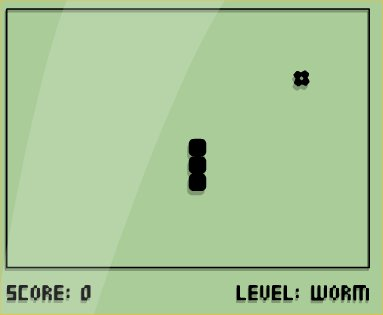
\includegraphics[width=0.7\textwidth]{images/snake.jpg}
  \end{figure}
  \end{center}
\end{frame}

\begin{frame}{Problem}
\begin{center}
	Can we measure the traits of a neural network in general?
	\begin{itemize}
	\item Application dependent
	\end{itemize}
\end{center}
\end{frame}

\begin{frame}{Traits}
  Solution: break down traits further
  \begin{itemize}
	\item Two neural networks have different traits if they for some input produce a different output.
  \end{itemize}
\end{frame}

\begin{frame}{Traits}
  Solution: break down traits further
  \begin{itemize}
	\item Two neural networks have different traits if they for some input produce a different output.
  \end{itemize}
    \vspace{30pt}
  Problem:
  \begin{itemize}
	\item We cannot try all possible inputs.
	\item Different outputs may behave the same.
  \end{itemize}
\end{frame}

\begin{frame}{Traits}
Observation:
\begin{itemize}
\item Some neural networks produce different outputs, but behave the same!
\end{itemize}
  \begin{figure}[p]
  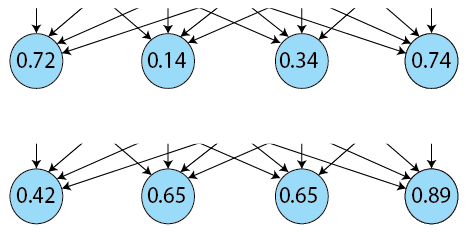
\includegraphics[width=0.8\textwidth]{images/whyhighestvalue.png}
  \end{figure}
\begin{itemize}
	\item Classification problems
	\item Decision problems
	\item $\cdots$
\end{itemize}
\end{frame}

\begin{frame}{Traits}
Observation:
\begin{itemize}
\item Some neural networks produce different outputs, but behave the same!
\end{itemize}
  \begin{figure}[p]
  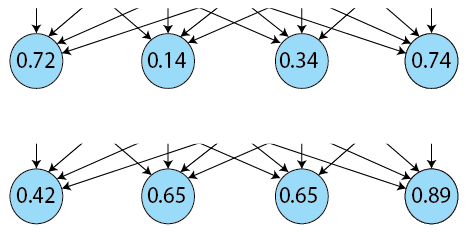
\includegraphics[width=0.8\textwidth]{images/whyhighestvalue.png}
  \end{figure}
\begin{itemize}
	\item Classification problems
	\item Decision problems
	\item $\cdots$
\end{itemize}
Let us only be concerned with the highest valued output neurons.
\end{frame}

\begin{frame}{NNTD}
\begin{center}
  \textbf{Input:} A set of neural networks.\\
  \textbf{Output:} A diversity measurement based on difference in \emph{traits}\\
  \vspace{30pt}
  \textbf{Method}:
  \begin{itemize}
  \item Calculate a large amount of random inputs
  \item For each input $\ran$:
  \begin{itemize}
	  \item Assign each neural network a species based on its output on $\ran$.
	  \item Calculate a diversity based on the distribution of individuals into species.
  \end{itemize}
  \item Return the average diversity for all random inputs.
  \end{itemize}
\end{center}
\end{frame}

\begin{frame}{NNTD}
\begin{center}
Calculate a large amount of random inputs (m-tuples) for the neural network architecture used
 \begin{figure}[p]
  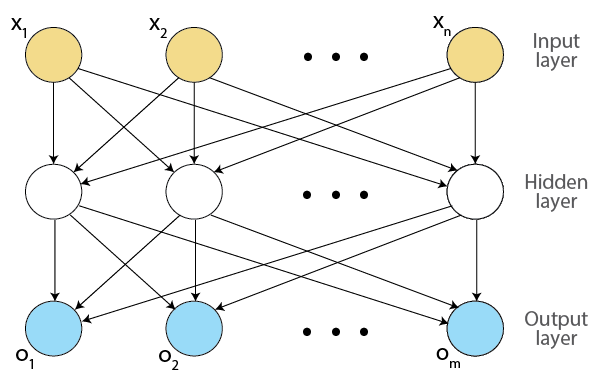
\includegraphics[width=0.7\textwidth]{images/neuralnetwork.png}
  \end{figure}
\end{center}
\end{frame}

\begin{frame}{NNTD}
\begin{center}
For each input:
  \begin{itemize}
      \item Calculate the output of all neural networks.
  \end{itemize}
   \begin{figure}[p]
  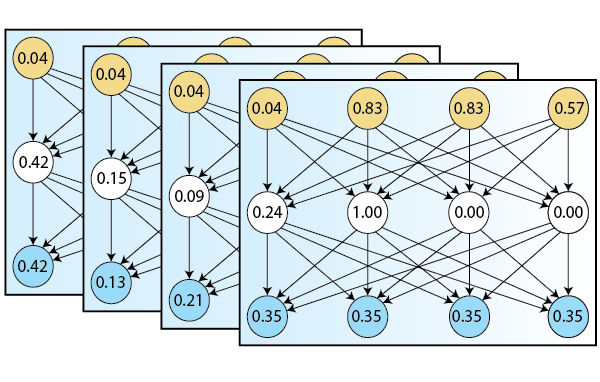
\includegraphics[width=0.7\textwidth]{images/neuralnetworkvalues.png}
  \end{figure}
\end{center}
\end{frame}

\begin{frame}{NNTD}
\begin{center}
For each input:
  \begin{itemize}
	  \item Distribute the neural networks into species based on their output.
  \end{itemize}
     \begin{figure}[p]
  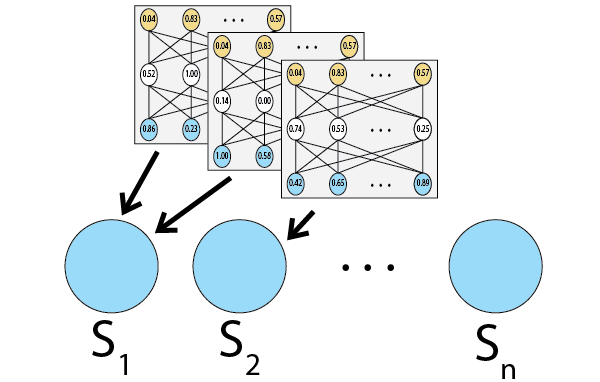
\includegraphics[width=0.7\textwidth]{images/speciesnn.png}
  \end{figure}
\end{center}
\end{frame}

\begin{frame}{Distribution of neural networks into species}
\begin{center}
Given neural network $f$ and input $\ran = (0.04, 0.83, 0.83, 0.57)$
  \begin{figure}[p]
  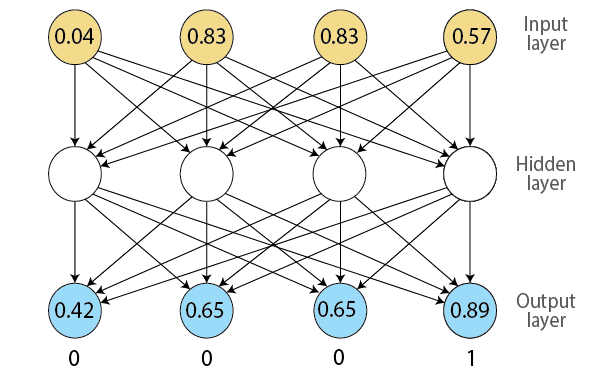
\includegraphics[width=0.75\textwidth]{images/nntdexample1.png}
  \end{figure}
We say that $f \in \speciesi{1}{\ran}$, because binary $\texttt{0001}$ is $1$ in decimal.
\end{center}
\end{frame}

\begin{frame}{Distribution of neural networks into species}
\begin{center}
Given neural network $f$ and input $\ran = (34, -5.7, 0, -4)$
  \begin{figure}[p]
  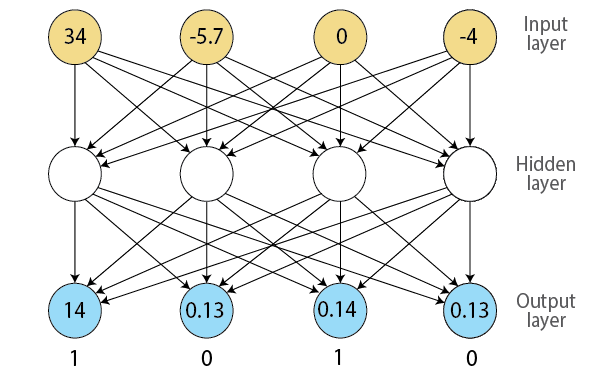
\includegraphics[width=0.75\textwidth]{images/nntdexample2.png}
  \end{figure}
We say that $f \in \speciesi{10}{\ran}$, because binary $\texttt{1010}$ is $10$ in decimal.
\end{center}
\end{frame}

\begin{frame}{Distribution of neural networks into species}
\begin{center}
Given neural network $f$ and input $\ran = (1, -1, 0, -1)$
  \begin{figure}[p]
  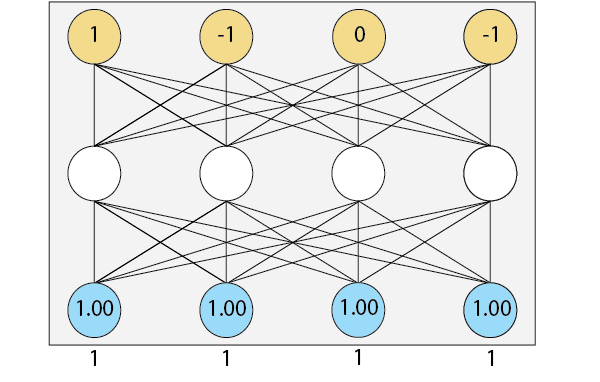
\includegraphics[width=0.75\textwidth]{images/nntdexample3.png}
  \end{figure}
We say that $f \in \speciesi{15}{\ran}$, because binary $\texttt{1111}$ is $15$ in decimal.
\end{center}
\end{frame}

\begin{frame}{Formally}
\begin{center}
If $b_{m}b_{m-1}\dots b_1$ is the binary representation of a number $i$, we define the species \speciesi{i}{\ran} to contain any neural network $\ind \in \indset$, that given $\ran$ as input satisfies
\begin{equation}
  \forall j \in \set{1, 2, \dots, m} \left(b_j \rightarrow (\nnout_j = h) \wedge \neg b_j \rightarrow (\nnout_j < h)\right)
\end{equation}
where $h = \max\set{\nnout_1, \nnout_2, \cdots, \nnout_b}$
\end{center}
\end{frame}

\begin{frame}{NNTD}
\begin{center}
For each input:
  \begin{itemize}
	  \item Calculate Simpson's Diversity Index based on the size of each species.
  \end{itemize}
     \begin{figure}[p]
  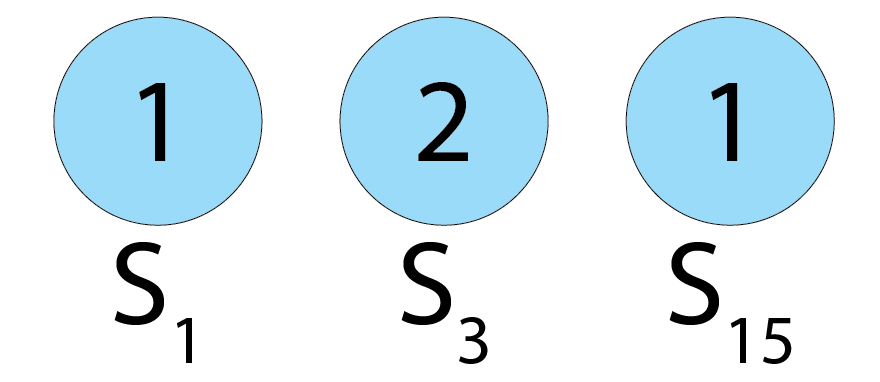
\includegraphics[width=0.4\textwidth]{images/speciessize.png}
  \end{figure}
\end{center}
\end{frame}

\begin{frame}{Simpson's Diversity Index}
\begin{center}
$r = (2.3, 3.4, -1.4, 3.2)$
  \begin{figure}[p]
  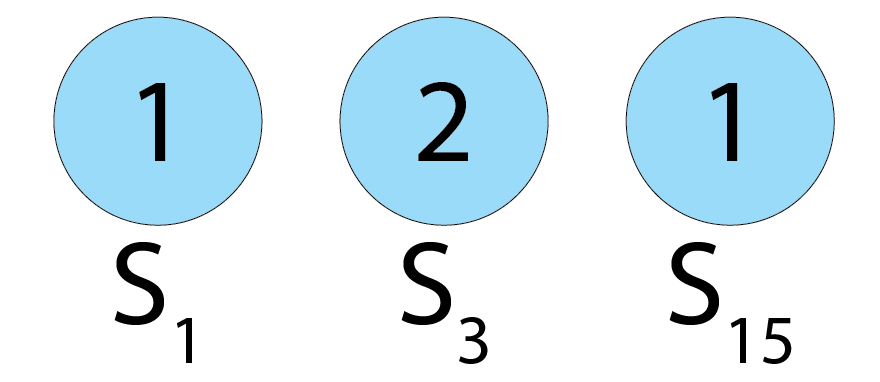
\includegraphics[width=0.4\textwidth]{images/speciessize.png}
  \end{figure}
\end{center}
\end{frame}

\begin{frame}{Simpson's Diversity Index}
\begin{center}
$r = (2.3, 3.4, -1.4, 3.2)$
  \begin{figure}[p]
  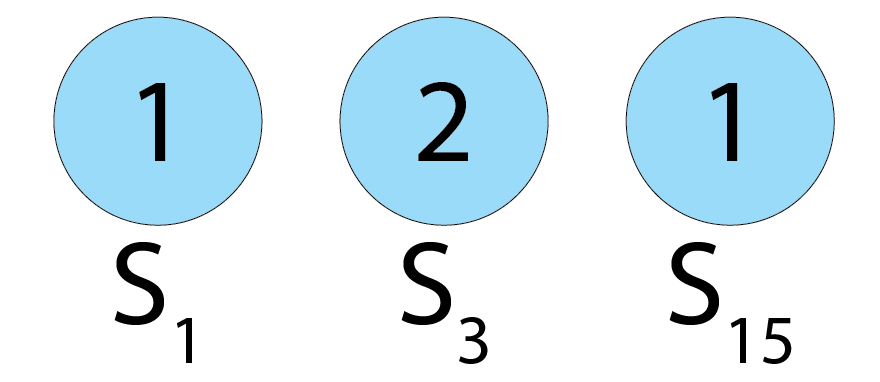
\includegraphics[width=0.4\textwidth]{images/speciessize.png}
  \end{figure}
\begin{equation}
D_r = 1 - \frac{\sum_{q \in \nemptyspeciesf{r}}\left(\sizeof{q}\left(\sizeof{q} - 1\right)\right)}{\indsetl\left(\indsetl - 1\right)}
\end{equation}
\end{center}
\end{frame}

\begin{frame}{Simpson's Diversity Index}
\begin{center}
$r = (2.3, 3.4, -1.4, 3.2)$
  \begin{figure}[p]
  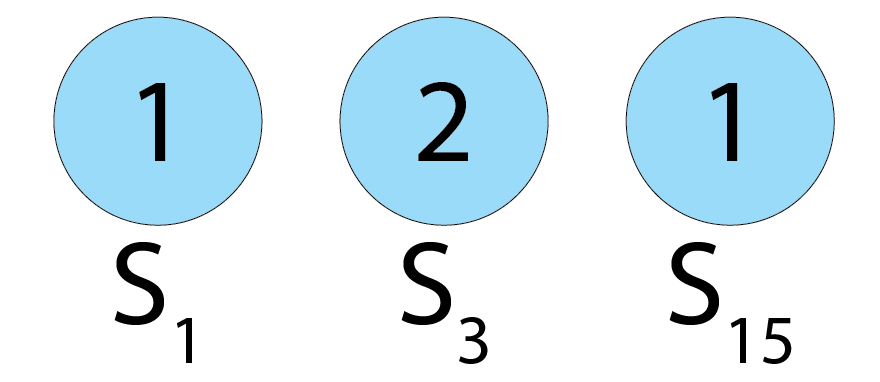
\includegraphics[width=0.4\textwidth]{images/speciessize.png}
  \end{figure}
\begin{equation}
D_r = 1 - \frac{\sum_{q \in \nemptyspeciesf{r}}\left(\sizeof{q}\left(\sizeof{q} - 1\right)\right)}{\indsetl\left(\indsetl - 1\right)}
\end{equation}
\begin{equation}\label{eq:nntd}
D_r = 1 - \frac{(2(2-1))+(1(1-1))}{3(3-1)} = \frac{2}{3}
\end{equation}
\end{center}
\end{frame}

\begin{frame}{NNTD}
\begin{center}
\textbf{NNTD:}\\
The average Simpson's Diversity Index for all random inputs.
\end{center}
\end{frame}





